\begin{figure}[H]
    \centering

\begin{tikzpicture}
\pgfplotsset{
    every axis/.style={ymin=0},
    width=0.22\textwidth,
    height=0.25\textheight,
    xtick={2, 3, 4, 5, 6, 7, 8, 9, 10},
    y axis style/.style={
    yticklabel style=#1,
    ylabel style=#1,
    y axis line style=#1,
    ytick style=#1}}
\begin{axis}[ scale only axis, ymin=500, xmin=2,xmax=10, axis y line*=left, xlabel=Number of Cores, ylabel=Duration (s), y axis style=green!75!black]
    \addplot[smooth, green!75!black, mark=o, draw] 
    coordinates 
    {
        (2,744.819)
        (3,693.8425)
        (4,675.287)
        (5,665.056)
        (6,654.828500)
        (7,660.632)
        (8,656.893)
        (9,660.654)
        (10,654.147)
    };
\end{axis}
%
\begin{axis}[ scale only axis, ymin=4000, xmin=2,xmax=10, axis y line*=right, axis x line=none, ylabel=DEC (j), y axis style=blue]%
    \addplot[smooth, blue, mark=x] 
    coordinates 
    {
        (2,6722.8189)
        (3,6437.60509)
        (4,6362.88499)
        (5,6336.77673028)
        (6,6296.86504)
        (7,6325.38972)
        (8,6253.5005)
        (9,6277.043141)
        (10,6241.910571)
    };
\end{axis}
%
\begin{axis}[red, scale only axis, ymin=3, xmin=2,xmax=10, axis y line*=right, axis x line=none, ylabel=DEC per second (w)]%
\pgfplotsset{every outer y axis line/.style={xshift=2cm}, every tick/.style={xshift=2cm}, every y tick label/.style={xshift=2cm} }
    \addplot[smooth, red ,mark=+] 
    coordinates 
    {
        (2,3.939189)
        (3,4.21989)
        (4,4.38183)
        (5,4.444353)
        (6,4.585327)
        (7,4.512795)
        (8,4.5118815)
        (9,4.4619282)
        (10,4.47744412)
    };
\end{axis} 

\end{tikzpicture}
    \caption{The evolution of the DEC (blue), DEC per second (red) and duration (green) as more cores are allocated to PCM on DUT 2. Note that the y-axis does not start at zero.}
    \label{fig:exp_3_dut_2_pcm_result}
\end{figure}